% For more detailed article preparation guidelines, please see:
% http://f1000research.com/author-guidelines

\documentclass[10pt,a4paper,twocolumn]{article}
\usepackage{f1000_styles}
\usepackage{gensymb}

%% Default: numerical citations
\usepackage[numbers]{natbib}

%% Uncomment this lines for superscript citations instead
% \usepackage[super]{natbib}

%% Uncomment these lines for author-year citations instead
% \usepackage[round]{natbib}
% \let\cite\citep

\usepackage{nicefrac}
\usepackage{url}
\def\UrlBreaks{\do\/\do-}

\begin{document}

\title{Evaluation of predicted medfly (\textit{Ceratitis capitata}) quarantine length in the United States utilizing degree-day and agent-based models}
% \titlenote{The title should be detailed enough for someone to know whether the article would be of interest to them, but also concise. Please ensure the broadness and claims within the title are appropriate to the content of the article itself.}

\author[1,2]{Travis C. Collier}
\author[1,3]{Nicholas C. Manoukis}
\affil[1]{Daniel K. Inouye US Pacific Basin Agricultural Research
Center (PBARC), United States Department of Agriculture,
Agricultural Research Service,
Hilo, Hawaii, 96720, USA}
\affil[2]{corresponding author; email: Travis.Collier@ARS.USDA.gov}
\affil[3]{email: Nicholas.Manoukis@ARS.USDA.gov}
% Please list all authors that played a significant role in the research involved in the article. Please provide full affiliation information (including full institutional address, ZIP code and e-mail address) for all authors, and identify who is/are the corresponding author(s).

\maketitle
\thispagestyle{fancy}

\begin{abstract}
Abstracts should be up to 300 words and provide a succinct summary of the article. Although the abstract should explain why the article might be interesting, care should be taken not to inappropriately over-emphasize the importance of the work described in the article. Citations should not be used in the abstract, and the use of abbreviations should be minimized. If you are writing a Research or Systematic Review article, please structure your abstract into Background, Methods, Results, and Conclusions.
\end{abstract}

\section*{Keywords}
%Please list up to eight keywords to help readers interested in your article find it more easily.
biosecurity, Mediterranean fruit fly, eradication, invasive pest, agriculture


\clearpage

%%%%%%%%%%%%%%%%%%%%%%%%%%%%%%%%%%%%%%%%%%%%%%%%%%%%%%%%%%%%%%%%%%%%%%%%%%%
TO REMOVE:

Take-homes:
\begin{enumerate}
\item There is significant variation in predicted quarantine length 
at different times and locations.
  \begin{enumerate}
  \item Captured by normals
  \item Climate
  \end{enumerate}
\item Variation in prediction within time / location (across years) 
is important.
  \begin{enumerate}
  \item Captured by day-of-year (between-year) variation
  \item Informs reliability of prediction
  \item Influenced by rare events (eg. cold snaps)
  \item Prediction based on normal temps vs normal 
  of predictions based on measured temps
  \end{enumerate}
\item DD vs ABS comparison
  \begin{enumerate}
  \item ABS is better behaved
    \begin{enumerate}
    \item Seasonal swings less dramatic; 
    Much less discontinuity at beginning of autumn 
    \item Smaller overall range
    \item Captures common-sense effects missed by DD: 
    eg. extreme cold kills
    \end{enumerate}
  \item Large disagreement between DD and ABS may indicate 
  DD prediction is unreliable/broken
  \item Variance in predictions should inform management and planning.
  ABS variance is easier to interpret (KFAT being a dramatic example).
  \end{enumerate}
\end{enumerate}

%%%%%%%%%%%%%%%%%%%%%%%%%%%%%%%%%%%%%%%%%%%%%%%%%%%%%%%%%%%%%%%%%%%%%%%%%%%

\section*{Introduction}

Invasions by insects, pathogens and pests increasingly appear to be a 
defining challenge of the 21\textsuperscript{st} century, facilitated by global connectivity, climatic shifts, and
other factors \cite{simberloff_impacts_2013} (find paper on number of invasive species).
Invasions by insects that do not become established are by their nature less
likely to be detected than those that are ``successful''
from the point of view of the insect. However, when the invading species
is of  environmental, human health or economic concern there is a greater
chance that cases of invasion followed by extirpation would be detected and
studied \cite{liebhold_population_2008}. Eradication of such insects
can be desirable and feasible \cite{Myers2000Eradication} depending on several
factors. One factor might be that the new environment is only marginally or 
seasonally suitable to the
invading insect, facilitating its eradication. Another is that the high cost of
allowing establishment leads
to extensive efforts for eradication. The invasion of
\emph{Anopheles gambiae} into Northeastern Brazil in the 1930's \cite{Soper1943Anopheles}
is one example of an invasive insect that was successfully eradicated 
primarily due to the second of these
reasons \cite{Causey1943Ecology,Killeen2002Eradication}.

In the case of \emph{An. gambiae} there have been no reports of
re invasion, but there are examples of insects that
recurrently invade areas outside their native range and are recurrently
extirpated within relatively few 
genrations. The Gypsy moth \emph{Lymantria dispar} in Canada
\cite{Gray2010Hitchhikers} is one such species, and arguably, the screwworm \emph{Cochlyomyia hominivorax}
around the area at the current northernmost edge of its range in Panama, and more recently in Florida,
\cite{Robinson2009Enabling} is another. (add citation on Florida)

One of the most important instances of repeated invasion and extirpation by an economically 
important pest is that of the \textit{Ceratitis capitata} (``Mediterranean fruit fly'', or `` Medfly'') 
in California.  
Though the establishment of these pests is disputed, a pattern of invasion, detection, and response, followed by no further detections for a long period, has been established over the last four decades. 
Some have argued that Medfly in California is an example of a ``metainvasion'', consisting of 
multiple sequential or
overlapping introductions \cite{Davies1999Bioinvasions}. Still other researchers have maintained 
that Medfly is repeatedly eradicated
from the state \cite{Haymer1997Genetic} or for different situations
in different regions of the state
\cite{Bonizzoni2001Microsatellite,Gasperi2002Genetic}. Medfly is occasionally found in 
other parts of the mainland US such as Florida (cite), and in other countries or areas that are considered 
free of the pest such as New Zealand (CHECK), and (some free areas here).

The response plan to Medfly in California, and the other ``free'' regions mentioned above, is extensive and 
 costly, including a quarantine \cite{Gilbert}. A practical and important problem 
is how long to maintain the countermeasures and quarantine following a last detection. 
Predicting the likely duration of required quarantines would help with
management decision making and planning,
including potential cost savings by having sufficient but not excessive
resources available. Currently most programs determine quarantine lengths by calculating the amount of
time required for a given number of generations to elapse under a thermal unit accumulation (``Degree day'')
physiological development model (CITE). Recently another approach to determining effective quarantine 
durations was introduced via Agent-Based Simulations \cite{Manoukis2014}. 

Agent-Based
Simulations (ABS) or models (also called ``Individual-Based'' or
	``Multi-Agent''), which can be minimally defined as those where
individuals are described as unique and autonomous, and where they usually
interact with each other and their environment on a local level
\cite{Railsback2011Agent}. Such simulations describe a system of
interest ``from the bottom up'': by implementing its constituent particles and
then observing the system behaviors and dynamics that result from those
particles interacting autonomously with their environment and often each other
\cite{Bonabeau2002Agent}. These models can include arbitrary amounts of complexity, limited
only by computational capacity, and are free of limitations imposed by mathematical 
tractability \cite{Huston1988New}.

While the freedom to include any degree of complexity
in an ABS comes at a cost
\cite{Deangelis1994Individual,Grimm1999Ten,Hales2003Model}, the pragmatic and
paradigmatic benefits of the Agent-Based mindset can be significant for diverse
areas of biology \cite{Macal2010Tutorial,Railsback2011Agent}, including biological
invasions. The benefits of the Agent-Based mindset have infrequently been 
applied to
questions of insect invasions \cite{vinatier2011factors} (but see \cite{crespo2011modeling}
for an example).
Here, we analysed the predicted quarantine length (PQL for short) 
for 11 sites in the continental United States
(figure \ref{fig:sitemap} and table \ref{tab:sites})
based on both the standard thermal accumulation degree day method\cite{ECY:ECY1969503514} 
as well as the MED-FOES\cite{manoukis_computer_2014} ABS  under sterile insect technique (SIT)\cite{??} eradication.

Seasonal variations dominate the variation in quarantine length predictions, 
so we aggregated the PQL values for each day of the year (Jan.\ 1, Jan.\ 2, ect.) 
across a large number of years (65 for most of locations) to produce normals.

\begin{figure}[ht!]
\centering
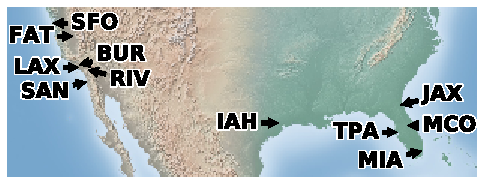
\includegraphics[width=0.4\textwidth]{figs/sitemap.pdf}
\caption{\label{fig:sitemap}Location of sites reported on.}
\end{figure}

\begin{table*}[ht!]
\hrule \vspace{0.1cm}
\caption{\label{tab:sites}Weather station (NOAA ISD) sites used.}
\centering
\begin{tabledata}{llllrrrl}
\header Callsign & Station Name & State & Latitude & Longitude & Elevation & Start year \\
\row KSFO &  SAN FRANCISCO INTERNATIONAL A &  CA &  +37.620 &  -122.365 &  2.4 & 1950 \\
\row KFAT &  FRESNO YOSEMITE INTERNATIONAL &  CA &  +36.780 &  -119.719 &  101.5 & 1950 \\
\row KBUR &     BURBANK-GLENDALE-PASA ARPT &  CA &  +34.201 &  -118.358 &  236.2 & 1973 \\
\row KLAX &  LOS ANGELES INTERNATIONAL AIR &  CA &  +33.938 &  -118.389 &  29.6 & 1950 \\
\row KRIV &         MARCH AIR RESERVE BASE &  CA &  +33.900 &  -117.250 &  468.2 & 1950 \\
\row KSAN &  SAN DIEGO INTERNATIONAL AIRPO &  CA &  +32.734 &  -117.183 &  4.6 & 1950 \\
\row KJAX &  JACKSONVILLE  INTERNATIONAL A &  FL &  +30.495 &  -81.694 &  7.9 & 1950 \\
\row KIAH &  G BUSH INTERCONTINENTAL AP/HO &  TX &  +29.980 &  -95.360 &  29.0 & 1970 \\
\row KMCO &  ORLANDO INTERNATIONAL AIRPORT &  FL &  +28.434 &  -81.325 &  27.4 & 1973 \\
\row KTPA &    TAMPA INTERNATIONAL AIRPORT &  FL &  +27.962 &  -82.540 &  5.8 & 1950 \\
\row KMIA &    MIAMI INTERNATIONAL AIRPORT &  FL &  +25.791 &  -80.316 &  8.8 & 1950 \\
\end{tabledata}
\end{table*}



\section*{Methods}
% Methods should include a brief discussion of allowances made (if any) for controlling bias or unwanted sources of variability, and the limitations of the datasets.


\begin{figure*}[ht!] % could add 'p' placement to allow it to be on its own page
\centering
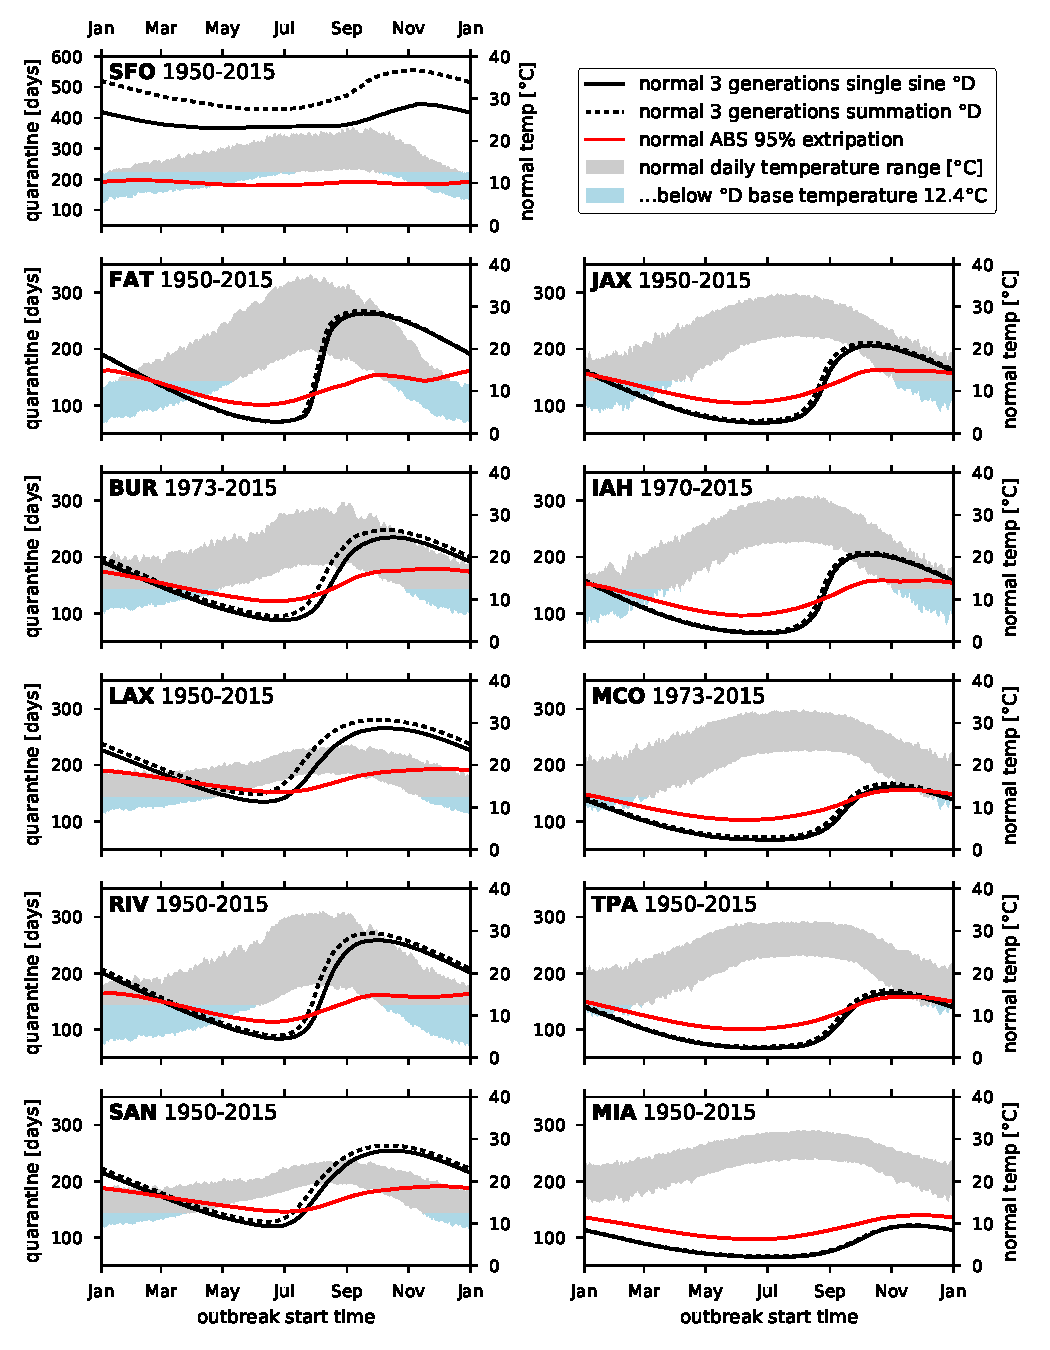
\includegraphics[width=1\textwidth]{figs/fig_main.pdf}
\caption{\label{fig:main_summary}Summary of normal quarantine length predictions for each site.
Year range of input temperature data used is inclusive.
All panels have identical limits except SFO quarantine.}
\end{figure*}



\subsection*{Sites and Temperature Data}
Hourly air temperature data for 11 sites was downloaded from 
NOAA's Integrated Surface Database (ISD) dataset\cite{smith_integrated_2011,NOAA_ISD_portal}.
The airport sites shown in figure \ref{fig:sitemap} 
were chosen for their biological relevance and 
availability of high quality hourly data over a long time frame.

Sites are referred to here by the last three letters of the callsign shown in table \ref{tab:sites}.
For 8 sites (SFO, FAT, LAX, RIV, SAN, JAx, TPA, and MIA), temperature data starting on 1950-01-01 was used.
The 3 other sites contained large ($>$ 14 days) gaps or other problems in the early years of their data,
so data starting on 1970-01-01 for IAH and 1973-01-01 for BUR and MCO was used.
For all sites, temperature data from the start date through 2017-05-15 was used
for quarantine length predictions for dates ranging from the start date for the site up to 2016-01-01.

Data was fetched and parsed using the \texttt{Fetching and parsing ISH.ipynb} program.
Records for the same station callsign were merged, since identification, format, 
and precise location of stations has changed over the years.
The data was then cleaned using the 
\texttt{Cleaning temperatures.ipynb} program by 
removing outliers, 
identifying large gaps ($>$ 3 hours), 
resampling to every hour on the hour using linear interpolation,
and filling the large gaps using day-over-day linear interpolation
(interpolating using values for the same hour of day from previous and following days).
The processing programs and resulting temperature datasets are 
provided in the Supplemental Materials.


\subsection*{Degree-Day Calculation}
Degree-days were computed by the single-sine method\cite{ECY:ECY1969503514}
using a base development temperature of 12.39\degree C (53.3\degree F) 
and 345.56 degree-days Celsius (DDc; 622 DDf) per generation 
following the standard required by California Department of Food and Agriculture
regulation 3406(b)\cite{CDFA_Medfly,3-CA-ADC-3406}.
%single-triangle\cite{10.2307/1933072}
Since we have hourly temperature data, we also calculated degree-days by simple summation
for comparison\cite{Roltsch1999}.
For each date, the number of days required to pass 3 generations of degree-day 
based life cycles was computed.
These calculations are implemented in \texttt{Temperature functions.ipynb} in the Supplemental Materials.


\subsection*{Agent-based Simulations: MED-FOES}

MED-FOES\cite{manoukis_computer_2014,manoukis_agent-based_2014} is 
an agent-based simulation explicitly modeling the eradication of a population of Medflies 
under inundative sterile male releases (aka: sterile insect technique or SIT).
A MED-FOES simulation models a single non-spatial population starting from a given age distribution 
and number of individuals through the time the population experiences extirpation when the last 
potentially fertile female dies or mates with a sterile male.
The simulation is parameterized on the initial population, additional mortality induced by control efforts,
the effectiveness of SIT, and a large number of biological parameters for which ranges are known from 
the literature, including temperature-dependent development and mortality.
The simulation is fed the same hourly timeseries of temperature values which was used for degree-day calculations
and updated in hourly time steps.

Due to the fact that only ranges are known for many of the parameters,
2500 individual MED-FOES simulations were run for each given start date at each site 
sampling different regions of parameter-space using a Latin Hypercube Sampling\cite{10.2307/1403510} procedure.
This set of simulations is referred to as a `run'.

Varying the start date for different simulations was achieved by simply 
starting at different points in the input temperature file; 
for this study a run starting every 7 days over the range of dates available for each site.
Each set of runs for a single site over a range of starting dates is referred to as a `runset'.
All runsets were conducted with the same input parameters aside from temperature.
Initial population numbers were chosen as a standard outbreak based upon several real 
outbreaks modeled previously\cite{manoukis_agent-based_2014}.

MED-FOES version 0.6.2 was run under OGS/Grid Engine 2011.11 on a CentOS 6.6 HPC cluster.
The MED-FOES code, configuration files, and helper scripts are provided in the Supplemental Materials.
Overall, we created 11 runsets (one for each site), 
each containing runs starting every 7 days over the input temperature data range for that site,
where each run contained 2500 individual simulations sampling different regions of 
biologically plausible parameter space.

The MED-FOES data is summarized here by the number of days from the start date required for
95\% of the simulations in a run to be eradicated, referred to as pe95.

\subsection*{Statistical analysis}

The main results reported here are `normals' in a meteorological sense of term,
but without the typical running mean smoothing which would complicate
interpretation of the results.
For a variable of interest (eg. temperature or PQL), 
all values for the same calendar day irrespective of year (eg. 20-July) are
aggregated and summary statistics such as mean, minimum, maximum, and standard deviation 
are computed for each aggregation.
Figure \ref{fig:main_summary} shows the minimum and maximum of the normals for temperatures
along with the mean of the normal PQL based on 3 generation degree day accumulation 
and MED-FOES 95\% extirpation.
Figures \ref{fig:DD_variation_summary} and \ref{fig:pe95_variation_summary} show the 
standard deviations ($\sigma$) of the normals for the degree day and MED-FOES based PQL.
\texttt{Temperature functions.ipynb} contains the code used to perform normal calculations, 
and the code generating these figures is \texttt{Summary Figures.ipynb}.

The results reported here are the normals of PQL computed using the full temperature time series
as opposed to computing PQL from the normal of the temperature timeseries.
While the latter is fairly common practice, it is not mathematically proper 
since, as with means, the normal of a function of $X$ is not generally equal to the function applied to the normal of $X$.
Additionally, by computing the normals of the predicted quarantine durations, 
we can investigate properties of the distribution of values as shown in 
figures \ref{fig:DD_variation_summary} and \ref{fig:pe95_variation_summary} and the ``supernorm" supplemental figures.


\section*{Results}

\begin{table}[htb!]
\hrule \vspace{0.1cm}
\caption{\label{tab:variance_captured_by_normal}
Percentage of PQL variance captured by the mean of the normal.  
DD PQL is the 3 generation single sine degree day based prediction, 
and pe95 is the MED-FOES agent-based simulation predictions.}
\centering
\begin{tabledata}{lrr}
\header & \multicolumn{2}{c}{$R^2$} \\
\header Site & DD PQL & pe95 \\
\row SFO &   9.12\% & 28.01\% \\
\row FAT &  93.93\% & 75.68\% \\
\row BUR &  90.71\% & 90.88\% \\
\row LAX &  80.17\% & 83.07\% \\
\row RIV &  92.23\% & 81.89\% \\
\row SAN &  80.99\% & 80.91\% \\
\row JAX &  96.45\% & 94.78\% \\
\row IAH &  95.10\% & 91.80\% \\
\row MCO &  94.62\% & 95.77\% \\
\row TPA &  91.91\% & 94.40\% \\
\row MIA &  88.42\% & 92.00\% \\
\end{tabledata}
\end{table}

There is significant variation in PQL across both time and location.
The temporal variation in PQL is dominated by a yearly cycle
which is characterized well by the normal values shown in figure \ref{fig:main_summary}.
Table \ref{tab:variance_captured_by_normal} shows the percentage of variance in 
quarantine length predictions which is captured by the mean of the normal yearly cycle (aka. $R^2$) for each site.
At all but one site, greater than 75\% of the variance in both degree day and MED-FOES based PQL
is accounted for by the mean normal, and the majority exceed 90\%.
SFO is an exception to the overall rule, with the mean normal accounting for only 9.1\% of the variation in 
degree day based PQL and 28.0\% of the MED-FOES based PQL.
This is also shown in the respective `supernorm' supplemental figures S?? and S??.

\subsection*{Seasonal dependence}

The seasonal variation, evidenced by the general shape of the curves shown in figure \ref{fig:main_summary}, 
is doubtless familiar to anyone engaged in medfly pest management.
Outbreaks starting in the late summer, autumn, or early winter will extend through relatively cold periods
where thermal dependent development will be slow and therefore extend the duration of quarantine required
for 3 generations of degree days to accumulate (referred to as DD PQL hereafter).
Similarly, outbreaks starting in the spring or early summer often lead to short quarantines due
to the relatively high temperatures.

This familiar pattern is also predicted by the MED-FOES ABS despite it being quite different in nature
from simple degree day accumulation.
However, the MED-FOES predictions (pe95) show a smaller seasonal swing.
pe95 generally predicts as smaller overall range of PQL,
with longer quarantines than DD PQL for spring and early summer outbreaks,
and shorter quarantines for late summer through early winter.

A particular feature of interest, shown most dramatically at FAT in figure \ref{fig:main_summary},
is that MED-FOES PQL often flattens out or even dips for quarantines starting in the late 
autumn or early winter.  This is due to relatively rare and brief cold-snaps,
normally lasting only a few hours, which increase mortality.
Since DD PQL does not account for mortality, it misses the effect of cold-snaps entirely.
This cold-snap effect is most clearly seen at more northern and 
more inland sites where cold-snaps are more likely: 
particularly FAT and RIV, but also BUR, LAX, JAX, and IAH.

\subsection*{Geographic dependence}

\begin{figure*}[ht!]
\centering
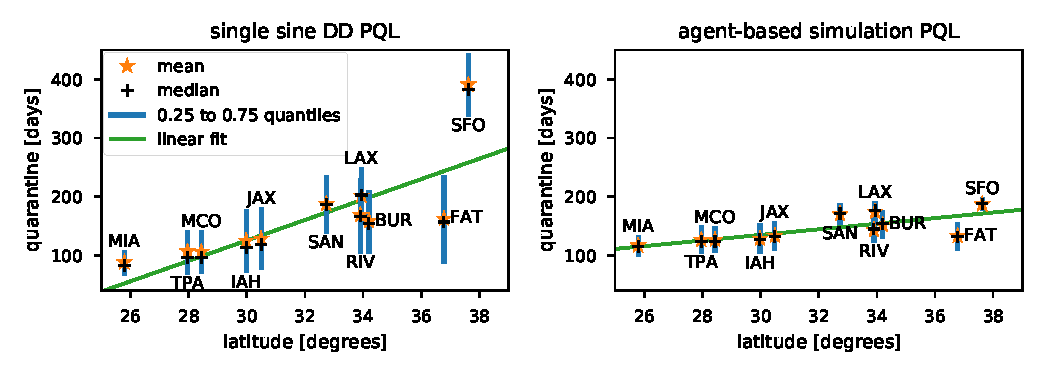
\includegraphics[width=0.9\textwidth]{figs/fig_latitude_trend_withSFO.pdf}
\caption{\label{fig:latitude_trend} Predicted quarantine length dependence on latitude.
For each site, the mean, median, and inter-quartile range are shown (similar to a boxplot).
An ordinary least-squares linear fit to the median values is shown by the green lines.
The left pane is for single sine degree day predictions,
and MED-FOES based predictions (pe95) in the right pane.
}
\end{figure*}

PQL generally shows a positive correlation with latitude\cite{??}.
Sites are ordered by latitude in the figures and tables.
As seen in figure \ref{fig:main_summary}, higher latitude sites tend to have longer PQL 
as well as larger seasonal swings for both DD and MED-FOES based predictions.

Figure \ref{fig:latitude_trend} shows the relationship between PQL and latitude.
An ordinary least squares fit to the median PQL at each site shows a significant slope for
both DD ($F{=}14.08$, $p{=}0.005$) and MED-FOES ($F{=}10.55$, $p{=}0.010$), but
the DD based predictions are more sensitive to latitude than MED-FOES
(coefficients of 17.39 and 4.78 respectively).
Additionally, the predictions for SFO, and to a lesser extent FAT, where the DD model for medfly appears to
break down are much better behaved under MED-FOES.

\subsection*{Variance and uncertainty}

\begin{figure*}[ht!]
\centering
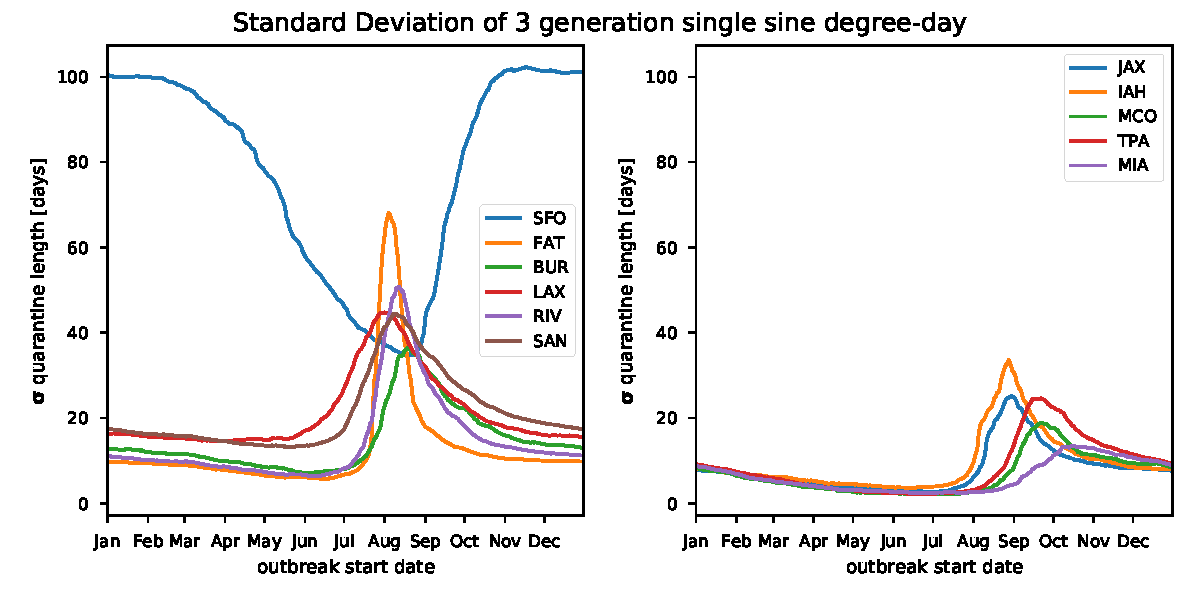
\includegraphics[width=0.9\textwidth]{figs/fig_BMDD_variation.pdf}
\caption{\label{fig:DD_variation_summary}Variation in quarantine length prediction 
based on 3 generations of single-sine degree day accumulation.}
\end{figure*}

\begin{figure*}[ht!]
\centering
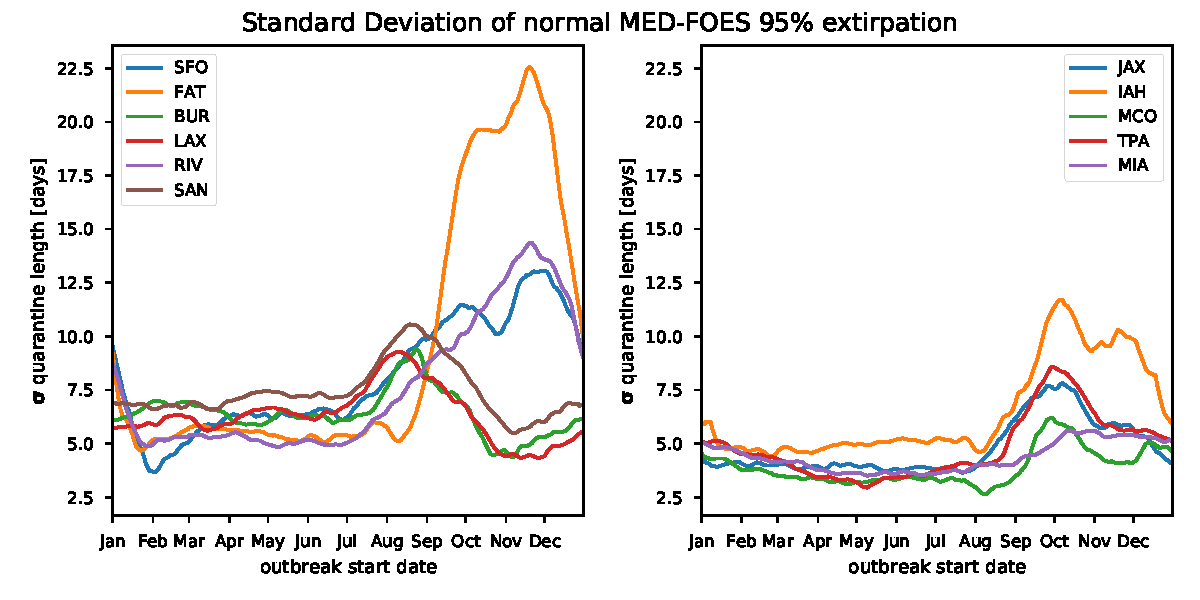
\includegraphics[width=0.9\textwidth]{figs/fig_pe95_variation.pdf}
\caption{\label{fig:pe95_variation_summary}Variation in quarantine length prediction 
based on 95\% of MED-FOES simulations showing extirpation.}
\end{figure*}


Figures \ref{fig:DD_variation_summary} and \ref{fig:pe95_variation_summary}
report the standard deviation ($\sigma$) of the normal for DD PQL and MED-FOES PQL respectively.
These indicate the year to year variability of the PQL for outbreaks starting at a
given time of the year and can be used to gauge the uncertainty of quarantine length predictions 
relative to the actual quarantine length which will be required.
Similar information is represented by the inter-quartile ranges shown in figure \ref{fig:latitude_trend} and 
the `supernorm' supplemental figures.
Those `supernorm' figures also show that the underlying distributions of PQL values are generally
not highly skewed, making $\sigma$ a realatively easy to interpret proxy for uncertainty.

Excluding SFO, the mean normal is a good predictor of DD PQL with values below 20 days
except for the late summer and early autumn, where variance increases 
due to quarantines extending through the cold season.
FAT and, to a lesser extent, RIV show this increase more dramtically, presumably due to their more 
aird/inland climates where both daily and seasonal temperature ranges are larger
(also see figure \ref{fig:main_summary}).
The standard deviation generally decreases with latitude.

The standard deviation in DD PQL for SFO shows a inversion of the seasonal trend othe sites exhibit.
This is due to the colder temperatures leading to extremely long degree day based quarantine predictions
frequently extending across two winter seasons.

The standard deviations of MED-FOES based PQL normals shown in figure \ref{fig:pe95_variation_summary}
are generally about \nicefrac{1}{2} as large as for DD based PQL.
This indicates that MED-FOES PQL not only shows less dramatic seasonal swings, but is also
produces more consistent predictions across years.
Values again generally decrease with latitude, but less consistently than DD PQL $\sigma$ of normals.
Also, unlike with the DD PQL, the results for SFO appear consistent with other sites.

A feature of interest is that BUR, LAX, and SAN all show an increase in the year to year variation
in MED-FOES PQL starting in July and extending through November, 
while that increase for all other sites starts in July or August 
but extends all the way to January or Feburary.
[@TCC: ANY CLUE WHY?]
Additionally, results for FAT show a sharp increase in uncertainty starting in September, which fits with the 
more aird/inland climate.  RIV shows a significant but more gradual increase.


\section*{Discussion}
% The discussion should include the implications of the article results in view of prior work in this field.




\section*{Conclusions}
Please state what you think are the main conclusions that can be realistically drawn from the findings in the paper, taking care not to make claims that cannot be supported.



\subsection*{Author contributions}
In order to give appropriate credit to each author of an article, the individual
contributions of each author to the manuscript should be detailed in this section. We
recommend using author initials and then stating briefly how they contributed.

\subsection*{Competing interests}
All financial, personal, or professional competing interests for any of the authors that
could be construed to unduly influence the content of the article must be disclosed and
will be displayed alongside the article.

\subsection*{Grant information}
Please state who funded the work discussed in this article, whether it is your employer,
a grant funder etc. Please do not list funding that you have that is not relevant to this
specific piece of research. For each funder, please state the funder’s name, the grant
number where applicable, and the individual to whom the grant was assigned.
If your work was not funded by any grants, please include the line: ‘The author(s)
declared that no grants were involved in supporting this work.’

\subsection*{Acknowledgements}
This section should acknowledge anyone who contributed to the research or the
article but who does not qualify as an author based on the criteria provided earlier
(e.g. someone or an organisation that provided writing assistance). Please state how
they contributed; authors should obtain permission to acknowledge from all those
mentioned in the Acknowledgements section.

Please do not list grant funding in this section.


{\small\bibliographystyle{unsrtnat}
\bibliography{main}}

% \bigskip
% References can be listed in any standard referencing style that uses a numbering system
% (i.e. not Harvard referencing style), and should be consistent between references within
% a given article.

% Reference management systems such as Zotero provide options for exporting bibliographies as Bib\TeX{} files. Bib\TeX{} is a bibliographic tool that is used with \LaTeX{} to help organize the user's references and create a bibliography. This template contains an example of such a file, \texttt{sample.bib}, which can be replaced with your own. Use the \verb|\cite| command  to create in-text citations, like this \cite{Smith:2012qr} and this \cite{Smith:2013jd}.


% See this guide for more information on BibTeX:
% http://libguides.mit.edu/content.php?pid=55482&sid=406343

% For more author guidance please see:
% http://f1000research.com/author-guidelines


% When all authors are happy with the paper, use the 
% ‘Submit to F1000Research' button from the menu above
% to submit directly to the open life science journal F1000Research.

% Please note that this template results in a draft pre-submission PDF document.
% Articles will be professionally typeset when accepted for publication.

% We hope you find the F1000Research Overleaf template useful,
% please let us know if you have any feedback using the help menu above.


\end{document}
